% M. S. Tsoeu (2011), University of Cape Town <mohohlo.tsoeu@uct.ac.za>

% This is a project report templace document created for EEE4022FS students at the University of Cape Town.
%
% This file should be is processed with ``pdflatex`` and might need a few modifications if a different processor is chosen.


\documentclass[a4paper,12pt]{report}

%Include packages you need to use here

\usepackage[top = 1in, bottom = 1in, left = 1in, right = 1in]{geometry}
\usepackage{graphicx}
\usepackage{fancyhdr}
\usepackage{amsmath, amsthm, amssymb}
\usepackage{lastpage}
\usepackage{subfigure}
\usepackage{lscape}
\usepackage{hyphenat}
\usepackage{setspace}
\usepackage{hyperref}
\usepackage{xcolor}
\usepackage{colortbl}
\usepackage{rotating}
\usepackage{multirow}
\usepackage{booktabs-de}
\usepackage{adjustbox}
\usepackage{graphicx}
%\usepackage{tabularx}


% Include page formatting here. 
\parskip = 6mm
\parindent = 0mm
\renewcommand{\headrulewidth}{0pt}
\rhead[]{\thesection}
\lhead[\thechapter]{}


\begin{document}
 
% This section formats the title page of the Report.
\thispagestyle{empty}
{\Huge \begin{center}
% Modify the line below to insert your title.
Virtual Tailor
\hrule 
% Modify the line below to insert your subtitle.
{\Large Human Body Parameter Determination using a Kinect Sensor}
\end{center}}

\vskip 5mm
\begin{center}
\- \- \- \- \- \- \- \- \- \- 
\includegraphics[scale = 0.3]{uctLogo.png}
\end{center}

\vskip 5mm
\begin{center}
Presented by:\\
Nevarr Pillay	% Insert your name here
\end{center}

\vskip 10mm
\begin{center}
Prepared for:\\
F. Nicolls\\ 		% Insert your supervisor's name here.
Dept. of Electrical and Electronics Engineering\\University of Cape Town
\end{center}


\vskip 10mm
\begin{center}
Submitted to the Department of Electrical Engineering at the University of Cape Town in partial
fulfilment of the academic requirements for a Bachelor of Science degree in Mechatronics.
\end{center}


\vskip 5mm
\begin{center}{\bf \today}
\end{center}

\newpage
\thispagestyle{empty}
\mbox{}

\newpage
\onehalfspacing
\nohyphens{
\thispagestyle{empty}
\vskip 40mm


% Please leave the declaration as it is (Standard UCT declaration).
{\Large Declaration}\\
\hrule

\vskip 10mm
\begin{enumerate}
\item I know that plagiarism is wrong. Plagiarism is to use another's work and pretend that it is one's
own.
\item I have used the IEEE convention for citation and referencing. Each contribution to, and quotation in,
this report from the work(s) of other people has been attributed, and has been cited and
referenced.
\item This report is my own work.
\item I have not allowed, and will not allow, anyone to copy my work with the intention of passing it off
as their own work or part thereof.
\end{enumerate}
\vskip 10mm
Signature:\ldots\ldots\ldots\ldots\ldots\ldots\ldots\ldots\ldots 
\\Nevarr Pillay 		% Chante this line to your name.
\vskip10mm
Date:\ldots\ldots\ldots\ldots\ldots\ldots\ldots\ldots\ldots\ldots .


\fancyfoot[C]{\thepage}
\pagestyle{plain}
\newpage
\pagenumbering{roman}
{\Large Acknowledgments}\\
\hrule

\newpage

{\Large Abstract}\\
\hrule

% Place your abstract here.
\begin{itemize}
\item Open the {\bf Project Report Template.tex} file and carefully follow the comments (starting with \%).
\item Process the file with {\bf pdflatex}, using other processors may need you to change some features such as graphics types.
\item Note the files included in the  {\bf Project Report Template.tex} (with the .tex extension excluded). You can open these files separately and modify their contents 
or create new ones.
\item Contact the latex namual for more features in your document such as equations, subfigures, footnotes, subscripts \& superscripts, special characters etc.
\item I recommend using the {\bf kile} latex IDE, as it is simple to use.
\end{itemize}


\newpage
\tableofcontents

%\newpage
%\listoffigures

%\newpage
%\listoftables

% Page formatting, to place section titles as headers of odd pages and Chapter titles as headers of even pages.
\newpage
\fancyhead[RE,LO]{}
\fancyhead[LE]{\leftmark}
\fancyhead[RO]{\rightmark}
\pagestyle{fancy}

\pagenumbering{arabic}

% THe files included below are .tex files containing the respective chapters these are already created in this package and you can add to or modify them.
\chapter{Introduction}

\section{Background to the study}
A very brief background to your area of research. Start off with a general introduction to the area and
then narrow it down to your focus area. Used to set the scene \cite{smt2011}.
\section{Objectives of this study}
\subsection{Problems to be investigated}
Description of the main questions to be investigated in this study.
\subsection{Purpose of the study}
Give the significance of investigating these problems. It must be obvious why you are doing this study
and why it is relevant.

\section{Scope and Limitations}
Scope indicates to the reader what has and has not been included in the study. Limitations tell the
reader what factors influenced the study such as sample size, time etc. It is not a section for excuses as
to why your project may or may not have worked.

\section{Plan of development}
Here you tell the reader how your report has been organised and what is included in each
chapter.

{\bf I recommend that you write this section last. You can then tailor it to your report.}

\chapter{Literature Review}

\begin{enumerate}
	\item [Technology] background 
	\item Depth Sensor technology + How Kinect works
	\item Point cloud map
	
	\item [Coding] references/Getting started
	\item Code references and and blog posts? 
	\item Previous example
	\item Hand Example
	
	\item [Mathematics] Used
	\item Papers on ellipse circumference
	
	\item [Improving] Accuracy
	\item Skeleton Joints filtering
	\item Error Model
	
	\item [Further] developments
	\item Augmented reality paper
	
	\item [Imaging] Processing Background
	\item Basics of an image - RGB
	\item Matlab
	\item Camera Model
	
	\item [Uncertainty] Measurements
	\item Gaussian 
	\item Triangular
\end{enumerate}

\section{Literature Guide}
\subsection{Getting Started}

\subsubsection{Non-Contact Human Body Parameter Measurement Based on Kinect Sensor \cite{nonContact2017}}

\paragraph{Overview}
This journal article provides an adequate base to understand many techniques used during this project. In the article, a similar project is explored in terms of using a Kinect to determine various personalized measurements. This includes measurements such as height, shoulder length, other key limb lengths and front perimeter measurements for the chest, stomach and waist. All of the work done in this article is similar to the work done in the initial stages of this project. The article also provides useful contextual information regarding the current use of this technology and background knowledge regarding the inner workings of the Kinect. 

\paragraph{Relevance}
The main contribution of this article was the background information it provided, together with the validation of certain aspects of the experiment methodology: 

\subparagraph{Background Theory}
This article provides a summary and overview of the process the Kinect utilises to retrieve data about a detected human. It explains the different sensors the Kinect posses, together with a basic understanding of the internal process required to track a skeleton and return information such as "Joint" position etc. This is explained in more detailed in Section \hl{(Reference to Middleware)}. It also provided an explanation of how pixels in the image plane are converted to real world positional points using information from both depth and colour frames. This is also explained in detail in Section \hl{(Depth - real conversion)}.

\subparagraph{Methodology}
This article was found after an initial strategy for calculating measurements was created. However, it served as a validation of the methods used, specifically with regards to using the Pythagorean Theorem in 3D space to calculate distances and for calculating the error between actual measurements and measurements obtained using the Kinect. These methods and the relevant equations are explained in Section \hl{(Measurement - Pyth + error)}. A method was also suggested for the calibration of results to improve their accuracy. However, this technique was not employed in this project. Reasons for the exclusion are given in Section \hl{(Design - No calibration or correction)}

\subsubsection{Real-Time Hands Detection in Depth Image by Using Distance with Kinect Camera \cite{handDetection2015}}

\paragraph{Overview}
This journal article explored various techniques to improve hand detection using a Kinect. The main focuses were in the areas of background removal, noise removal and feature extraction. Traditional image processing techniques require a large amount of processing power and often produced ambiguous results, with regards to feature extraction, and were prone to noise. Introduction of the Kinect allowed for the use of depth data to reduce the computational power needed and to improve the accuracy of the results. A large section of the paper was dedicated to "Shadow Removal", which is the process of removing depth data unavailable due to an object obstructing the emitted Infrared Rays. "Shadow" was determined to be a significant source of noise in the depth data and its removal improved the accuracy of the system.    

\paragraph{Relevance}
This article was very specific to the detection of hands and therefore its use was limited. However, valuable insights were gained regarding the "Shadow Removal" and Background Removal processes implemented \hl{(Classifier Maybe)}:

\subparagraph{Shadow Removal}
The intricacies of Kinect in creating a depth image using its IR Emitter and IR Camera were explored in more detail. This further expanded on the inner workings of the Kinect and contributed to Section \hl{(Depth Image Creation - Kinect)}. Additionally, this brought attention to a significant source of noise in the depth image and provided a method to improve the accuracy of measurement results. This method is explored in Section \hl{(Rec - Noise Removal)}

\subparagraph{Background Removal}
This article detailed a method of Background Removal that did not utilise the BackgroundRemoval API available in the Kinect for Windows SDK. This method provides an alternative method for background that could be investigated if the BackgroundRemoval API does not provide the desired results. This is explored further in Section \hl{(Rec - Background Removal)}

\subsubsection{A Real Time Virtual Dressing Room Application using Kinect \cite{virtualDress2012}}

\paragraph{Overview}
This report details and explains an approach used to create a virtual dressing room. The end result was an application that allowed a user to see what clothing would look like by augmenting it onto their body. This was executed in a three part process of user extraction, user tracking and clothing mapping. A Kinect sensor was used to extract the user from the background using depth images and user information. The Kinect was also used to track the skeleton of the user and create a coordinate system on which the virtual clothing could be mapped. Lastly, information including joint orientation and key body lengths were used to augment the clothing model onto the body.  

\paragraph{Relevance}
This report details and explains a possible extension on this project that would be very useful in a production level solution. 

\subparagraph{Augmented Reality}
The virtual dressing room proposed in the report is foundational solution using augmented reality and requires further work and research in itself. However, once it is improved to a level sufficient for implementation, it would significantly improve the customer experience. This is envisioned to be used after the customer uses the system, proposed in this report, to determine their full body parameters. The customer would be able to use the virtual dressing room to get an accurate understanding of how different clothes would look on them, without needing to physically try them on. This is expanded on in Section\hl{(Rec - Virtual Dressing Room)} 

\subsubsection{Performance Evaluation of the 1st and 2nd Generation Kinect For Multimedia Applications \cite{kinectComp2011}}

\paragraph{Overview}
This report evaluates the performance of the Xbox 360 Kinect (First Generation - v1) and the Xbox One Kinect (Second Generation - v2). The launch of the Kinect v1 in 2010 was revolutionary as it made depth acquisition more affordable and accessible to a wide spectrum of users. Further excitement was created when Microsoft launched the Kinect v2 only three years later. However, the technology used for depth acquisition in the second generation Kinect was completely different to that of the first. The first generation Kinect utilised structured light which is a well known technology used by industry grade laser scanners for 3D construction. The second generation Kinect, on the other hand, uses a Time-Of-Flight (ToF) camera. This drastic changed piqued interest about the performance difference between the sensors and their ideal applications. Consequently, this report is among many written to quantify the difference. 

\paragraph{Relevance}
This report provided in depth knowledge about the principle of operation of the Kinect used in this project, together with its successor. This information contributed both to the background theory for the Kinect's operation and to component selection.

\subparagraph{Background Theory}
The first generation Kinect which is utilised in this project, operates on a principle known as structured light. This knowledge is provides an essential base of understanding that allows for the effect manipulation of data retrieved from the sensor. Also, it provides more information regarding the limitations of the technology. As such, ideal operating conditions can be determined which greatly aids in experimental design. More detail is given in Section \hl{(Sensor Background)}.

\subparagraph{Component Selection}
This report aided in the selection of a component for the design. The results yielded that the second generation Kinect on average performs better than the first generation Kinect. However, a large amount of performance testing was done in extreme conditions such as in direct sunlight, in darkness, at far distances etc. Consequently, significant disparity in the performance occurred mostly in these special conditions. For the purposes and operating conditions of the project, the first generation Kinect is sufficient. Elaboration into the evaluation between the two sensors is done in Section \hl{Component Selection} 

\subsubsection{Kinect for Windows Sensor Components and Specifications}

\paragraph{Overview}
This technical documentation provided by Microsoft details the components that comprise the Kinect sensor and its specifications. This provides background information regarding the types of information it provides and a high-level description of how the sensor operates.

\paragraph{Relevance}
This high-level description of the Kinect provides the foundation of background information that is required before development with the Kinect can take place. 

\subparagraph{Background Theory}
The essential information retrieved from this document include a description of each component segment of the Kinect and their respective specifications. The key details retrieved are as follows: 
\begin{itemize}
	\item The resolution of the RGB camera
	\item The operation of the depth sensor
	\item Frame rates for the depth and colour stream
	\item Viewing angle or field of view of the Kinect
	\item Vertical tilt range
	\item The accelerometer used to detect to determine the orientation of the Kinect 
\end{itemize}

\subsubsection{Coordinate Spaces}

\paragraph{Overview}
This technical documentation provided by Microsoft details the coordinate spaces for the three streams of data available - Colour, Depth and Skeleton. This provides background information explains how to interpret the data explains the manner in which it is stored. It also provides a brief introduction to how to use the API to transform data between the different spaces.

\paragraph{Relevance}
This description expands on the introductory theory provided on the component composition of the Kinect. This forms the reference used for digital representation of real world information captured by the relevant sensing components. It delves deeper into the intricacies of each of the data types and provides the base for interpreting and manipulating the data algorithmically. 

\subparagraph{Colour Space}
 

\subparagraph{Depth Space}

\subparagraph{Skeleton Space}


It forms the reference that is be used when  description of each component segment of the Kinect and their respective specifications. The key details retrieved are as follows: 
\begin{itemize}
	\item The resolution of the RGB camera
	\item The operation of the depth sensor
	\item Frame rates for the depth and colour stream
	\item Viewing angle or field of view of the Kinect
	\item Vertical tilt range
	\item The accelerometer used to detect to determine the orientation of the Kinect 
\end{itemize}

Definitions!!!!!!!!!!!!!!!!!\\
Accuracy\\
Precision\\
Kinect\\
Volunteer\\
Operator\\
IR - Infrared Rays\\


When writing your review start of with the general concepts and move to the more specific aspects
explaining the necessary theory as you go. This section is NOT a copy and paste from others work or a
rewrite-but-change-one-word section. I suggest you read all your material, and then put it down and
write this section, referring back to the work only when you need to check something.

See your PCS textbook for more details on how to write a literature review.

If you include a figure or a table in your text please see the example in Fig. \ref{fig:model} as to how to caption it.
Please make sure that all text in your figures is readable and that you reference your figures if they are
from another source.

\begin{figure}[ht]
\centering
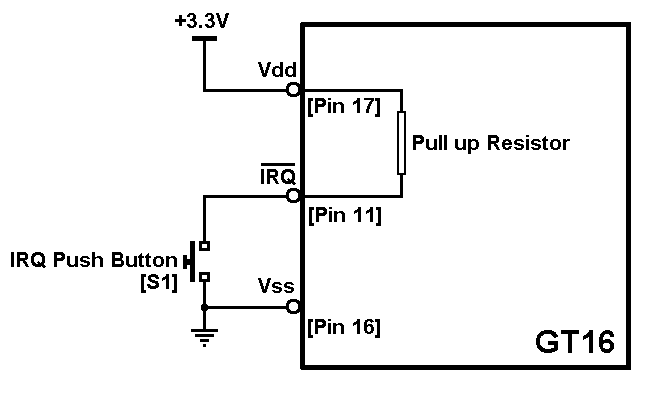
\includegraphics[width=0.7\textwidth]{model.png}
\caption{A block diagram illustrating the connections to the IRQ pin on the MCS08GT16A microcontroller (Please
note that your headings should be short descriptions of what is in the diagram not simply the figure title)}
\label{fig:model}
\end{figure}


\chapter{Solution Design}

\section{Implementation Design}
1) Online profile of people - Used for online shopping and retail shops\\
2) Take measurements at a retailer - Virtual Dressing room - A part of the shopping experience and will reduce hassle of trying on clothes\\
3) Amount wasted in trying on clothes or online returns?\\
4) Could be used for personalised tailoring
5) Example of UI - Explanation of how it works

\section{Component Selection}
1) Choice of Kinect\\
2) Choice of Windows SDK\\

\section{Algorithm Design}
1) Windows examples used - Background Removal, Colour Stream and Skeleton Tracking - NB - Why BackgroundRemoval instead of own method
3D Points - No calibration

2) Run through of algorithm
- Background Removed frame
- Send image to separate class for processing
- Create array with background removed pixels
- Draw skeleton on image
- Create axes for measurement - Perpendicular or straight depending on particular measurement

\section{Experimental Design}
- Constraints - Men, distance from Kinect, Number of views, 3D Modelling
- UI to run simulated dressing room
- Volunteer to pose as instructed by person controlling UI
- Take measurement of front
- Take left
- Take back
- Take right 
- At each point, take actual readings with uncertainty
- Note: Did not use correction in \cite{nonContact2017}
- For one volunteer, take 5 readings in relatively the same pose - Determine uncertainty 
\chapter{Methodology}

This is what I did to test and confirm my hypothesis.


You may want to split this chapter into sub chapters depending on your design. I suggest you change
the title to something more specific to your project.

This is where you describe your design process in detail, from component/device selection to actual
design implementation, to how you tested your system. Remember detail is important in technical
writing. Do not just write I used a computer give the computer specifications or the oscilloscopes part
number. Describe the system in enough detail so that someone else can replicate your design as well
as your testing methodology.

If you use or design code for your system, represent it as flow diagrams in text.

\begin{enumerate}
\item This is a bullet point test
\item I hope this works
	
\end{enumerate}	

The aim of this project was to create a system that enabled the measurement of different parts of a human body
\chapter{Results}
These are the results obtained from the investigation outlined in \ref{methodology}. Seven volunteers were used in determining the accuracy of the system. They were first measured by the system and then their physical measurements were obtained for comparison. This chapter explores the results obtained for the measurement of the extremities of a human body and the modelling of 3D body parts, together with the observed performance of the user interface respectively.

\section{Length and Extremity Measurement}

This section begins with a presentation of the overall results of the system and a comparison with the aim of the investigation. Subsequent subsections present further performance of specific areas of the system that form the basis of analysis presented in Chapter \ref{analysis}. These sections focus on the following major areas of the system:

\begin{itemize}
	\item The accuracy of measuring key lengths.
	\item The accuracy of each view of measurement (Front, Left, Back and Right) for measuring extremities.
	\item The accuracy of measuring the extremity of each individual limb.
	\item The impact that clothing worn by a person being measured has on the system's accuracy.
	\item Other empirical insights obtained through use and observation of the system. 
\end{itemize}


\subsection{Overall Results}
Below is a summary of the aggregate accuracy of the system and the accuracy per volunteer, together with their personal characteristics. (Table \ref{tab:overallAccuracy})
 
 % Table generated by Excel2LaTeX from sheet 'Overall'
 \begin{table}[htbp]
 	\centering
 	\caption{Overall results of accuracy of system per volunteer}
 	\begin{tabularx}{\textwidth}{|YY|YYY|}
 		\toprule
 		\multicolumn{1}{|Y|}{\textit{\textbf{Volunteer Number}}} & \textit{\textbf{Average Error}} & \multicolumn{1}{Y|}{\textit{\textbf{Build}}} & \multicolumn{1}{Y|}{\textit{\textbf{Height}}} & \textit{\textbf{Clothing}} \\
 		\midrule
 		\multicolumn{1}{|Y|}{\textit{\textbf{1}}} & 28.44\% & \multicolumn{1}{Y|}{Athletic} & \multicolumn{1}{Y|}{Tall} & Tight \\
 		\midrule
 		\multicolumn{1}{|Y|}{\textit{\textbf{2}}} & 17.27\% & \multicolumn{1}{Y|}{Athletic} & \multicolumn{1}{Y|}{Average} & Tight \\
 		\midrule
 		\multicolumn{1}{|Y|}{\textit{\textbf{3}}} & 16.45\% & \multicolumn{1}{Y|}{Athletic} & \multicolumn{1}{Y|}{Tall} & Vest \\
 		\midrule
 		\multicolumn{1}{|Y|}{\textit{\textbf{4}}} & 40.75\% & \multicolumn{1}{Y|}{Slim} & \multicolumn{1}{Y|}{Average} & Loose \\
 		\midrule
 		\multicolumn{1}{|Y|}{\textit{\textbf{5}}} & 20.72\% & \multicolumn{1}{Y|}{Big} & \multicolumn{1}{Y|}{Average} & Loose \\
 		\midrule
 		\multicolumn{1}{|Y|}{\textit{\textbf{6}}} & 19.60\% & \multicolumn{1}{Y|}{Slim} & \multicolumn{1}{Y|}{Short} & Tight \\
 		\midrule
 		\multicolumn{1}{|Y|}{\textit{\textbf{7}}} & 18.83\% & \multicolumn{1}{Y|}{Big} & \multicolumn{1}{Y|}{Average} & Vest \\
 		\midrule
 		\multicolumn{5}{|Y|}{} \\
 		\midrule
 		\multicolumn{2}{|V|}{\textit{\textbf{Total Average Error}}} & \multicolumn{3}{W|}{23.15\%} \\
 		\bottomrule
 	\end{tabularx}%
 	\label{tab:overallAccuracy}%
 \end{table}%
 
As seen in Table \ref{tab:overallAccuracy}, despite the average error of some individual volunteers being outside the desired range of 25\% accuracy, the total average error of the system is 23.15\%. 

\subsection{Length Performance}
Seen below in Table \ref{tab:lengthResults} are the results of the average accuracy of key lengths obtained after measuring the volunteers in the "Front" view. These lengths are used using joint locations determined by the Kinect's Skeleton Tracking. 
\hl{Insert reference}

% Table generated by Excel2LaTeX from sheet 'Overall'
\begin{table}[htbp]
	\centering
	\caption{Results of the average accuracy of key lengths per volunteer}
	\begin{tabularx}{\textwidth}{|Y|Y|Y|Y|Y|Y|}
		\toprule
		\textit{\textbf{Volunteer Number}} & \textit{\textbf{Left Arm}} & \textit{\textbf{Right Arm}} & \textit{\textbf{Left Leg}} & \textit{\textbf{Right Leg}} & \textit{\textbf{Torso}} \\
		\midrule
		\textit{\textbf{1}} & 6.59\% & 4.35\% & 5.64\% & 3.38\% & 19.52\% \\
		\midrule
		\textit{\textbf{2}} & 11.88\% & 7.66\% & 3.22\% & 10.53\% & 9.55\% \\
		\midrule
		\textit{\textbf{3}} & 12.75\% & 19.49\% & 0.54\% & 0.99\% & 12.15\% \\
		\midrule
		\textit{\textbf{4}} & 8.76\% & 10.64\% & 1.43\% & 0.07\% & 0.51\% \\
		\midrule
		\textit{\textbf{5}} & 2.25\% & 10.17\% & 8.35\% & 7.79\% & 5.64\% \\
		\midrule
		\textit{\textbf{6}} & 4.57\% & 3.08\% & 2.36\% & 3.17\% & 9.38\% \\
		\midrule
		\textit{\textbf{7}} & 2.29\% & 2.54\% & 0.27\% & 2.47\% & 2.98\% \\
		\midrule
		\textit{\textbf{Total Avg Error}} & \textit{\textbf{7.01\%}} & \textit{\textbf{8.27\%}} & \textit{\textbf{3.12\%}} & \textit{\textbf{4.06\%}} & \textit{\textbf{8.53\%}} \\
		\bottomrule
	\end{tabularx}%
	\label{tab:lengthResults}%
\end{table}%

As seen in Table \ref{tab:lengthResults}, all length measurements fell well within the desired accuracy range of 20\%. The most accurate length on average was the "Left Leg" with an accuracy of 3.12\% and the least accurate length on average was the Torso with an accuracy of 8.53\%.

\subsection{View Performance}

Each "view" (Front, Left, Back or Right) of the system has a unique set of characteristics. It is useful to investigate the performance of each of them to better understand their effectiveness in the system as a whole. 

Seen below in Table \ref{tab:viewResults} are the results of the average accuracy of each view obtained after measuring the volunteers in each of the respective views. 

% Table generated by Excel2LaTeX from sheet 'Overall'
\begin{table}[htbp]
	\centering
	\caption{Results of the average accuracy of each view per volunteer}
	\begin{tabularx}{\textwidth}{|Y|Y|Y|Y|Y|}
		\toprule
		\textit{\textbf{Volunteer Number}} & \textit{\textbf{Front}} & \textit{\textbf{Left}} & \textit{\textbf{Back}} & \textit{\textbf{Right}} \\
		\midrule
		\textit{\textbf{1}} & 21.82\% & 29.90\% & 32.61\% & 31.04\% \\
		\midrule
		\textit{\textbf{2}} & 16.58\% & 15.81\% & 20.45\% & 14.60\% \\
		\midrule
		\textit{\textbf{3}} & 17.27\% & 19.01\% & 15.53\% & 13.37\% \\
		\midrule
		\textit{\textbf{4}} & 35.58\% & 58.15\% & 33.58\% & 44.77\% \\
		\midrule
		\textit{\textbf{5}} & 21.06\% & 10.39\% & 24.92\% & 23.47\% \\
		\midrule
		\textit{\textbf{6}} & 11.65\% & 44.58\% & 14.09\% & 17.07\% \\
		\midrule
		\textit{\textbf{7}} & 20.72\% & 19.51\% & 20.60\% & 12.06\% \\
		\midrule
		\textit{\textbf{Total Avg Error}} & \textit{\textbf{20.67\%}} & \textit{\textbf{28.19\%}} & \textit{\textbf{23.11\%}} & \textit{\textbf{22.34\%}} \\
		\bottomrule
	\end{tabularx}%
	\label{tab:viewResults}%
\end{table}%

As seen in Table \ref{tab:viewResults}, the accuracy of the views in descending order are as follows:

\begin{enumerate}
	\item Front
	\item Right
	\item Back
	\item Left
\end{enumerate}

The only view that performed outside the desired accuracy range of 25\% was the "Left" view with an average accuracy of 28.19\%. The Front view performed the best with an accuracy of 20.67\%.  

\subsection{Limb Performance}
Each extremity being measured is subtly different due to various factors such as position, orientation and size. Therefore, understanding how the system performs in these different cases is useful.

Due to the large number of measurements being taken, the results have been split up in terms of upper and lower body measurements.
 
Below is a summary of the aggregate accuracy of the system in measuring upper body limbs per volunteer: (Table \ref{tab:upperBodyResults})

% Table generated by Excel2LaTeX from sheet 'Overall'
\begin{table}[htbp]
	\centering
	\caption{Results of the average accuracy of Upper Body Limbs}
	\begin{tabularx}{\textwidth}{|Y|Y|Y|Y|Y|Y|}
		\toprule
		\textit{\textbf{Volunteer Number}} & \textit{\textbf{Chest}} & \textit{\textbf{Upper Left Arm}} & \textit{\textbf{Lower Left Arm}} & \textit{\textbf{Upper Right Arm}} & \textit{\textbf{Lower Right Arm}} \\
		\midrule
		\textit{\textbf{1}} & 49.50\% & 29.90\% & 10.10\% & 26.35\% & 11.02\% \\
		\midrule
		\textit{\textbf{2}} & 27.84\% & 23.16\% & 9.84\% & 17.74\% & 13.24\% \\
		\midrule
		\textit{\textbf{3}} & 14.58\% & 10.99\% & 24.14\% & 7.33\% & 12.27\% \\
		\midrule
		\textit{\textbf{4}} & 79.55\% & 12.20\% & 26.74\% & 33.79\% & 5.47\% \\
		\midrule
		\textit{\textbf{5}} & 45.85\% & 21.22\% & 8.41\% & 15.16\% & 14.82\% \\
		\midrule
		\textit{\textbf{6}} & 23.39\% & 6.64\% & 15.91\% & 8.46\% & 8.63\% \\
		\midrule
		\textit{\textbf{7}} & 30.70\% & 12.34\% & 12.71\% & 12.02\% & 7.95\% \\
		\midrule
		\textit{\textbf{Total Avg Error}} & \textit{\textbf{38.77\%}} & \textit{\textbf{16.64\%}} & \textit{\textbf{15.41\%}} & \textit{\textbf{17.26\%}} & \textit{\textbf{10.48\%}} \\
		\bottomrule
	\end{tabularx}%
	\label{tab:upperBodyResults}%
\end{table}%

As seen in Table \ref{tab:upperBodyResults}, measurements of the lower and upper portions of both arms fell well within the desired accuracy of 25\%. However, the chest measurements seemed to be significantly more inaccurate with an average of 38.77\%, which is far outside the desired range.

Below is a summary of the aggregate accuracy of the system in measuring lower body limbs per volunteer: (Table \ref{tab:lowerBodyResults})

% Table generated by Excel2LaTeX from sheet 'Overall'
\begin{table}[htbp]
	\centering
	\caption{Results of the average accuracy of Lower Body Limbs}
	\begin{tabularx}{\textwidth}{|Y|Y|Y|Y|Y|Y|}
		\toprule
		\textit{\textbf{Volunteer Number}} & \textit{\textbf{Waist}} & \textit{\textbf{Upper Left Leg}} & \textit{\textbf{Lower Left Leg}} & \textit{\textbf{Upper Right Leg}} & \textit{\textbf{Lower Right Leg}} \\
		\midrule
		\textit{\textbf{1}} & 32.09\% & 31.47\% & 13.58\% & 28.07\% & 44.04\% \\
		\midrule
		\textit{\textbf{2}} & 25.36\% & 15.32\% & 14.18\% & 13.21\% & 6.61\% \\
		\midrule
		\textit{\textbf{3}} & 20.51\% & 13.09\% & 24.62\% & 20.01\% & 10.12\% \\
		\midrule
		\textit{\textbf{4}} & 80.55\% & 13.36\% & 27.94\% & 25.40\% & 48.15\% \\
		\midrule
		\textit{\textbf{5}} & 26.74\% & 16.08\% & 8.56\% & 24.17\% & 15.81\% \\
		\midrule
		\textit{\textbf{6}} & 35.04\% & 20.78\% & 43.78\% & 9.58\% & 17.38\% \\
		\midrule
		\textit{\textbf{7}} & 19.53\% & 23.78\% & 22.77\% & 26.17\% & 16.17\% \\
		\midrule
		\textit{\textbf{Total Avg Error}} & \textit{\textbf{34.26\%}} & \textit{\textbf{19.13\%}} & \textit{\textbf{22.20\%}} & \textit{\textbf{20.95\%}} & \textit{\textbf{22.61\%}} \\
		\bottomrule
	\end{tabularx}%
	\label{tab:lowerBodyResults}%
\end{table}%

As seen in Table \ref{tab:lowerBodyResults}, measurements of the lower and upper portions of both legs fell within the desired accuracy of 25\%. This was similar to the behaviour of the arm measurements, mentioned above. However, they seemed to be slightly more inaccurate with all of the leg measurements having an accuracy tolerance of more than 19\%, whereas the arms all fell within 17.5\%. The waist measurement also followed the behaviour of the chest measurement above, where seemed to be significantly more inaccurate than the leg measurements. It had an average accuracy tolerance of 34.26\%, which is also outside the desired range.

\subsection{Impact of Clothing}

The nature of the system is such that it is sensitive to clothing worn by the measured party. One aim of the system, as stipulated, in section \ref{methodologyHypothesis}, was to make the system more robust to clothing, such that the results are less prone to error.

As such, each of the above measurement results tables have been adjusted to remove the effects of clothing. This has been done by analysing the data set after volunteers with observed "loose" clothing were removed.

Below is the clothing adjusted version of Table \ref{tab:overallAccuracy}. 

% Table generated by Excel2LaTeX from sheet 'Overall'
\begin{table}[htbp]
	\centering
	\caption{Overall results of accuracy of system per volunteer after adjustments for clothing}
	\begin{tabularx}{\textwidth}{|YY|YYY|}
		\toprule
		\multicolumn{1}{|Y|}{\textit{\textbf{Volunteer Number}}} & \textit{\textbf{Average Error}} & \multicolumn{1}{Y|}{\textit{\textbf{Build}}} & \multicolumn{1}{Y|}{\textit{\textbf{Height}}} & \textit{\textbf{Clothing}} \\
		\midrule
		\multicolumn{1}{|Y|}{\textit{\textbf{2}}} & 17.27\% & \multicolumn{1}{Y|}{Athletic} & \multicolumn{1}{Y|}{Average} & Tight \\
		\midrule
		\multicolumn{1}{|Y|}{\textit{\textbf{3}}} & 16.45\% & \multicolumn{1}{Y|}{Athletic} & \multicolumn{1}{Y|}{Tall} & Vest \\
		\midrule
		\multicolumn{1}{|Y|}{\textit{\textbf{6}}} & 19.60\% & \multicolumn{1}{Y|}{Slim} & \multicolumn{1}{c|}{Short} & Tight \\
		\midrule
		\multicolumn{1}{|Y|}{\textit{\textbf{7}}} & 18.83\% & \multicolumn{1}{Y|}{Big} & \multicolumn{1}{c|}{Average} & Vest \\
		\midrule
		\multicolumn{5}{|Y|}{} \\
		\midrule
		\multicolumn{2}{|V|}{\textit{\textbf{Total Error Average}}} & \multicolumn{3}{W|}{\textit{\textbf{18.04\%}}} \\
		\bottomrule
	\end{tabularx}%
	\label{tab:overallResultsClothingAdj}%
\end{table}%

It is clear from Table \ref{tab:overallResultsClothingAdj} that the system performs significantly better when loose clothing is not worn by the volunteer. The new overall average accuracy of the system improved to 18.04\%, which is well within the desired range of 25\%. 

The same behaviour can be observed for the accuracy of the views and the different limbs.

In the adjusted version of Table \ref{tab:viewResults} (Table \ref{tab:viewResultsClothingAdj}), the performance of all the views improve. Additionally, the "Left" view now also falls within the desired 25\% range and all the other views fall within 18\%. 

% Table generated by Excel2LaTeX from sheet 'Overall'
\begin{table}[htbp]
	\centering
	\caption{Results of the average accuracy of each view per volunteer after adjustments for clothing}
	\begin{tabularx}{\textwidth}{|Y|Y|Y|Y|Y|}
		\toprule
		\textit{\textbf{Volunteer Number}} & \textit{\textbf{Front}} & \textit{\textbf{Left}} & \textit{\textbf{Back}} & \textit{\textbf{Right}} \\
		\midrule
		\textit{\textbf{2}} & 16.58\% & 15.81\% & 20.45\% & 14.60\% \\
		\midrule
		\textit{\textbf{3}} & 17.27\% & 19.01\% & 15.53\% & 13.37\% \\
		\midrule
		\textit{\textbf{6}} & 11.65\% & 44.58\% & 14.09\% & 17.07\% \\
		\midrule
		\textit{\textbf{7}} & 20.72\% & 19.51\% & 20.60\% & 12.06\% \\
		\midrule
		\textit{\textbf{Total Avg Error}} & \textit{\textbf{16.55\%}} & \textit{\textbf{24.73\%}} & \textit{\textbf{17.67\%}} & \textit{\textbf{14.27\%}} \\
		\bottomrule
	\end{tabularx}%
	\label{tab:viewResultsClothingAdj}%
\end{table}%

As for the adjusted upper and lower body measurements (Table \ref{tab:upperBodyResultsClothingAdj} and Table  \ref{tab:lowerBodyResultsClothingAdj} respectively), all of the measurements, except for the "Lower Left Leg" measurement (increased to 26.34\% which is outside the desired range) either improved in accuracy or remained within 1\% of its previous accuracy. The "Chest" measurement is now within the desired accuracy range of 25\% with a value of 24.13\%. The "Waist" measurement also greatly improved, however, is still narrowly outside the desired range with an accuracy of 25.11\%   

% Table generated by Excel2LaTeX from sheet 'Overall'
\begin{table}[htbp]
	\centering
	\caption{Results of the average accuracy of Upper Body Limbs after adjustments for clothing}
	\begin{tabularx}{\textwidth}{|Y|Y|Y|Y|Y|Y|}
		\toprule
		\textit{\textbf{Volunteer Number}} & \textit{\textbf{Chest}} & \textit{\textbf{Upper Left Arm}} & \textit{\textbf{Lower Left Arm}} & \textit{\textbf{Upper Right Arm}} & \textit{\textbf{Lower Right Arm}} \\
		\midrule
		\textit{\textbf{2}} & 27.84\% & 23.16\% & 9.84\% & 17.74\% & 13.24\% \\
		\midrule
		\textit{\textbf{3}} & 14.58\% & 10.99\% & 24.14\% & 7.33\% & 12.27\% \\
		\midrule
		\textit{\textbf{6}} & 23.39\% & 6.64\% & 15.91\% & 8.46\% & 8.63\% \\
		\midrule
		\textit{\textbf{7}} & 30.70\% & 12.34\% & 12.71\% & 12.02\% & 7.95\% \\
		\midrule
		\textit{\textbf{Total Avg Error}} & \textit{\textbf{24.13\%}} & \textit{\textbf{13.28\%}} & \textit{\textbf{15.65\%}} & \textit{\textbf{11.39\%}} & \textit{\textbf{10.52\%}} \\
		\bottomrule
	\end{tabularx}%
	\label{tab:upperBodyResultsClothingAdj}%
\end{table}%

% Table generated by Excel2LaTeX from sheet 'Overall'
\begin{table}[htbp]
	\centering
	\caption{Results of the average accuracy of Lower Body Limbs after adjustments for clothing}
	\begin{tabularx}{\textwidth}{|Y|Y|Y|Y|Y|Y|}
		\toprule
		\textit{\textbf{Volunteer Number}} & \textit{\textbf{Waist}} & \textit{\textbf{Upper Left Leg}} & \textit{\textbf{Lower Left Leg}} & \textit{\textbf{Upper Right Leg}} & \textit{\textbf{Lower Right Leg}} \\
		\midrule
		\textit{\textbf{2}} & 25.36\% & 15.32\% & 14.18\% & 13.21\% & 6.61\% \\
		\midrule
		\textit{\textbf{3}} & 20.51\% & 13.09\% & 24.62\% & 20.01\% & 10.12\% \\
		\midrule
		\textit{\textbf{6}} & 35.04\% & 20.78\% & 43.78\% & 9.58\% & 17.38\% \\
		\midrule
		\textit{\textbf{7}} & 19.53\% & 23.78\% & 22.77\% & 26.17\% & 16.17\% \\
		\midrule
		\textit{\textbf{Total Avg Error}} & \textit{\textbf{25.11\%}} & \textit{\textbf{18.24\%}} & \textit{\textbf{26.34\%}} & \textit{\textbf{17.24\%}} & \textit{\textbf{12.57\%}} \\
		\bottomrule
	\end{tabularx}%
	\label{tab:lowerBodyResultsClothingAdj}%
\end{table}%


\subsection{Other Empirical Observations}

Apart from the above presented tables of results, other observations were made of the system during its use. These observations are explained in each of the following subsections:

\subsubsection{Background Removal Error} 
There were instances where the Background Removal functionality of the Kinect performed with error. These errors presented themselves in two manners:


\begin{figure}[ht]
	\centering
	{%
		\setlength{\fboxsep}{0pt}%
		\setlength{\fboxrule}{1pt}%
		\fbox{
	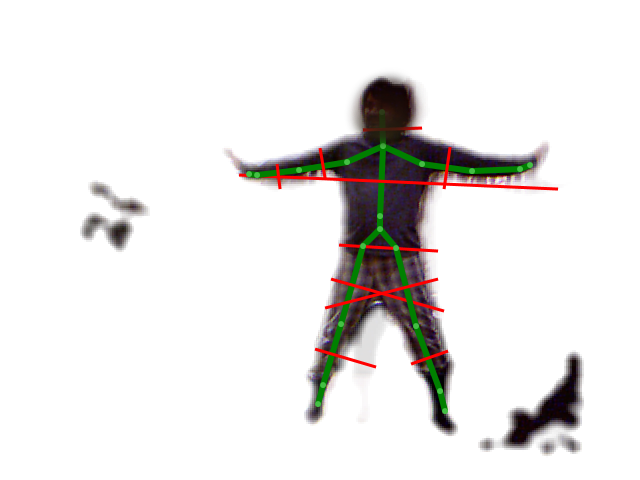
\includegraphics[width=0.7\textwidth]{ErrorExample_Blurred.png}
	}}
	\caption{An example of failures of extremity measurements due to background removal and padding errors detected in early testing}
	\label{fig:errorExample}
\end{figure}

\begin{figure}[ht]
	\centering
	%{%
	%	\setlength{\fboxsep}{0pt}%
	%	\setlength{\fboxrule}{1pt}%
	%	\fbox{
	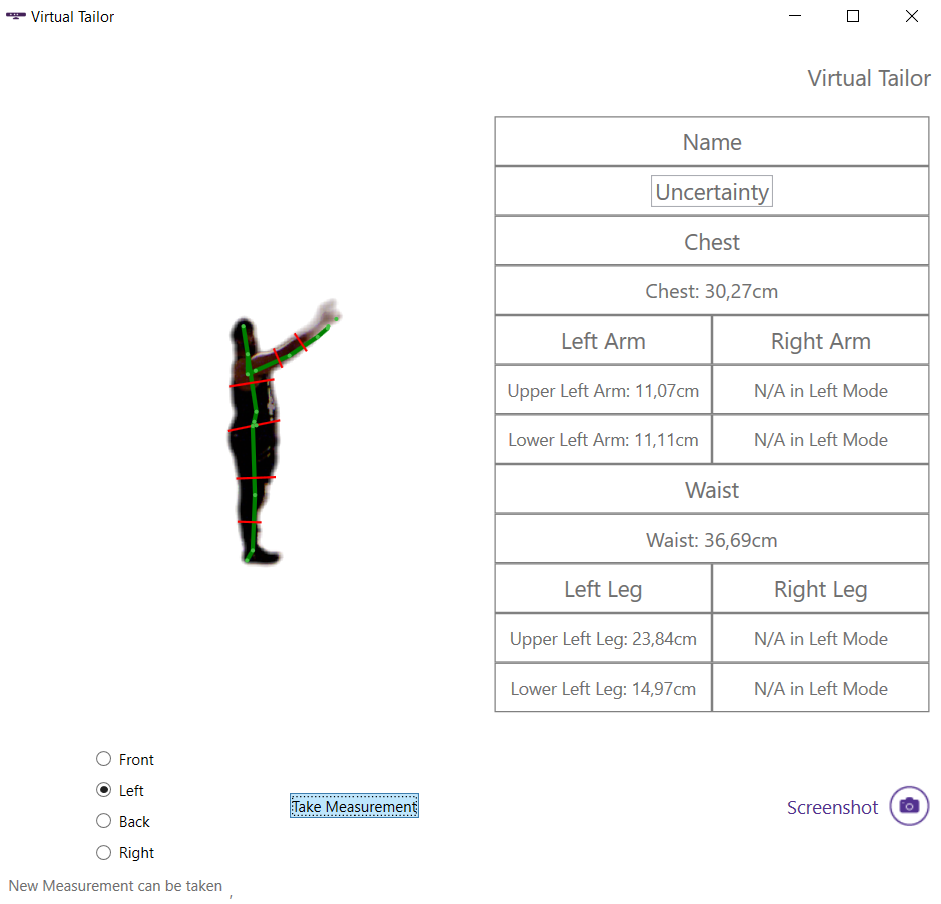
\includegraphics[width=0.7\textwidth]{Uncertainty_Left4.png}
	%}}
	\caption{An example of trailing pixels detected by background removal that forms part of padding errors}
	\label{fig:uncertaintyLeft4}
\end{figure}

\begin{figure}[ht]
	\centering
	%{%
	%	\setlength{\fboxsep}{0pt}%
	%	\setlength{\fboxrule}{1pt}%
	%	\fbox{
	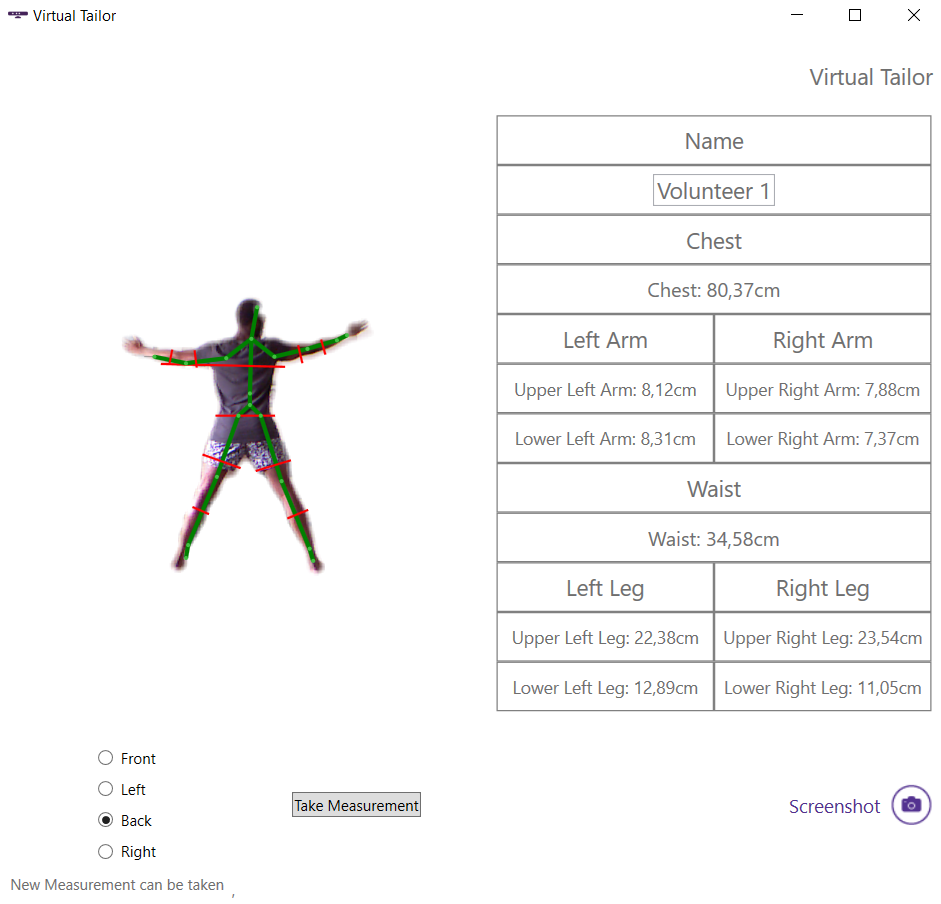
\includegraphics[width=0.7\textwidth]{Volunteer1_Back.png}
	%}}
	\caption{An example of failures of extremity measurements due to background removal and padding errors during final testing}
	\label{fig:volunteer1Back}
\end{figure}

\begin{figure}[ht]
	\centering
	%{%
	%	\setlength{\fboxsep}{0pt}%
	%	\setlength{\fboxrule}{1pt}%
	%	\fbox{
	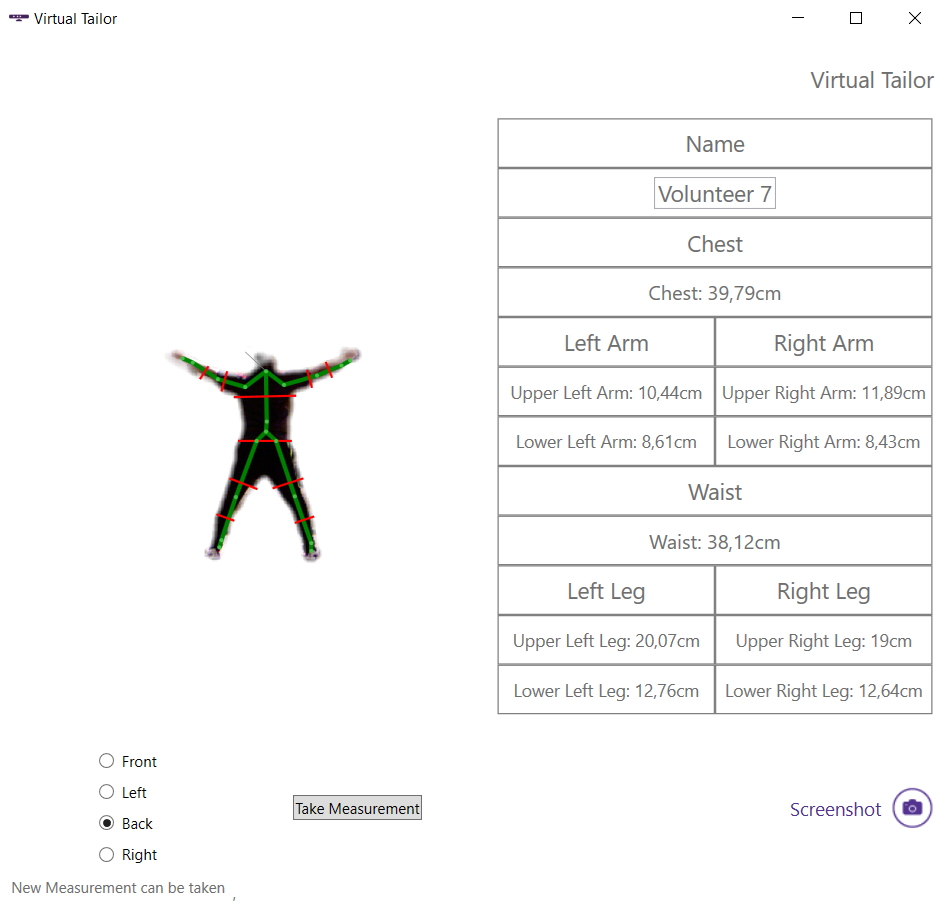
\includegraphics[width=0.7\textwidth]{Volunteer7_Back.png}
	%}}
	\caption{An example of the presence of a background removal error relating to incorrect pixel removal during final testing}
	\label{fig:volunteer7Back}
\end{figure}

\paragraph{Extra Padding}
During early and final testing of the system, it was observed that the output background removed picture had extra padding around the detected human in some instances. This extra padding consisted of background pixels that should have been removed. 

An example of an early test with the above error can be seen in Figure \ref{fig:errorExample}. In this image, it can be clearly seen that extra background pixels have been included in regions under the outstretched arms, on the sides of the torso and underneath the groin. 

An additional caveat to the above error was also detected. It was observed that when the detected human was processed while moving, trailing pixels from the previous position would be included in the image and form part of the padding.

This was present in both early testing and final testing. In Figure \ref{fig:errorExample}, mentioned above, this can be clearly seen as the right leg has a "ghost" or "trailing" leg present. An example of a final test with trailing pixels can be seen in Figure \ref{fig:uncertaintyLeft4}. In this image, careful inspection of the extended hand reveals that trailing pixels are present due to movement of the detected human.

\paragraph{Incorrect Pixel Removal}
The other error present as a result of the Background Removal functionality is the incorrect pixel removal of pixels that form part of the detected human. The parts of the body that suffered the most frequently from this error are the parts at the extremes (E.g. Head, hands, "feet, etc.). Additionally, the view in which incorrect pixel removal from the "Head" was the most prevalent, was the "Back" view. 

An example of a final test with incorrect pixel removal can be seen in Figure \ref{fig:volunteer7Back}. Careful inspection of this image reveals that pixels that form part of the head and hands of the detected human have been incorrectly removed. 

\subsubsection{Overlap Error}
It was observed that occasionally, the system failed to detect a correct extremity. As mentioned in \hl{Insert Reference}, measuring extremities assumes that an outline of a limb will be against a background and will thus be removed  due to an overlap. 


8) Empirical Insights - Trying to determine a correct measurement, Legs not together, length of people, skinny person, skeleton not perfectly fitting, background edges not perfect \\

5) Uncertainty model\\

6) Circumference results - Ellipse
7) Circumference results - Rectangle


9) Improved UI - trying to determine perfect pose
10) Data Set Analysis\\

Test of Table \ref{tab:testTable} added to results

% Table generated by Excel2LaTeX from sheet 'Volunteer 1'
\begin{table}[htbp]
	\centering
	\caption{Add caption}
	%\begin{adjustbox}{width=\textwidth}	
	%\resizebox{\textwidth}{!}{
	\begin{tabularx}{\textwidth}{|X|X|X|X|X|X|X|X|X|X|X|}
		\toprule
		& Chest & Waist & Upper Left Arm & Lower Left Arm & Upper Right Arm & Lower Right Arm & Upper Left Leg & Lower Left Leg & Upper Right Leg & Lower Right Leg \\
		\midrule
		\rowcolor[rgb]{ .573,  .816,  .314} Front & 38.92 & 38.27 & 7.97  & 9.28  & 7.09  & 7.27  & 24.72 & 12.55 & 24.38 & 12.02 \\
		\midrule
		\rowcolor[rgb]{ 0,  .69,  .941} Front & 38    & 31    & 11.5  & 9     & 12    & 7.5   & 15.5  & 10.5  & 15.5  & 10.5 \\
		\midrule
		Error & 2.42\% & 23.45\% & -30.70\% & 3.11\% & -40.92\% & -3.07\% & 59.48\% & 19.52\% & 57.29\% & 14.48\% \\
		\midrule
		\rowcolor[rgb]{ .573,  .816,  .314} Left  & 28.73 & 31.96 & 7.39  & 8.73  & \#N/A & \#N/A & 20.05 & 12.55 & \#N/A & \#N/A \\
		\midrule
		\rowcolor[rgb]{ 0,  .69,  .941} Left  & 20    & 20.5  & 11    & 7.5   & \#N/A & \#N/A & 14.5  & 11.5  & \#N/A & \#N/A \\
		\midrule
		Error & 43.65\% & 55.90\% & -32.82\% & 16.40\% & \#N/A & \#N/A & 38.28\% & 9.13\% & \#N/A & \#N/A \\
		\midrule
		\rowcolor[rgb]{ .573,  .816,  .314} Back  & 80.37 & 34.58 & 8.12  & 8.31  & 7.88  & 7.37  & 22.38 & 12.89 & 23.54 & 11.05 \\
		\midrule
		\rowcolor[rgb]{ 0,  .69,  .941} Back  & 35    & 30    & 11    & 7.5   & 11.5  & 9.5   & 15    & 11.5  & 14.5  & 11.5 \\
		\midrule
		Error & 129.63\% & 15.27\% & -26.18\% & 10.80\% & -31.48\% & -22.42\% & 49.20\% & 12.09\% & 62.34\% & -3.91\% \\
		\midrule
		\rowcolor[rgb]{ .573,  .816,  .314} Right & 25.68 & 29.42 & \#N/A & \#N/A & 9.8   & 8.78  & \#N/A & \#N/A & 17.38 & 24.58 \\
		\midrule
		\rowcolor[rgb]{ 0,  .69,  .941} Right & 21    & 22    & \#N/A & \#N/A & 10.5  & 9.5   & \#N/A & \#N/A & 17    & 11.5 \\
		\midrule
		Error & 22.29\% & 33.73\% & \#N/A & \#N/A & -6.67\% & -7.58\% & \#N/A & \#N/A & 2.24\% & 113.74\% \\
		\bottomrule
	\end{tabularx}%
	%}
	%\end{adjustbox}
	\label{tab:testTable}%
\end{table}%

\section{3D Modelling}

\section{User Interface Observations}

\chapter{Discussion}

Here is what the results mean and how they tie to existing literature...

Discuss the relevance of your results and how they fit into the theoretical work you described in your
literature review.

\chapter{Conclusions}

\subsection{Overall}
From the performance of the system created and tested, it is clear that an implementable solution using a Kinect sensor is certainly possible. Based on the results analysed, the system was able to determine majority of the measurements and most with an accuracy within the desired range. That being said, a large amount of further research and development is needed before this solution become practical. Additionally, the data set used was effective in identifying trends, however, a larger data set should be used and analysed determine the legitimacy of these trends. Each of the following subsections provide conclusions on their respective functional block of the system. Chapter \ref{recommendations} suggests possible solutions or further areas of exploration to many problems expressed in this chapter. 

\subsection{Extremity Measurements}
This formed the crux of the project and for the most part, performed within expected ranges: Average accuracy, length accuracy, view accuracy and limb accuracy all fell within the desired ranges. However, these ranges used were relatively large and were used to prove the "rough" efficacy of the system. For a solution to be viable, very accurate results would be required and the maximum allowed error would be in the region of $<5\%$. 

Additionally, the system exhibited a significant weakness to clothing being worn. In terms of the envisioned implementation, customers would be more likely to use the system if they did not need to remove their clothes as they may feel uneasy about being exposed in front of a data collection device. Therefore, the system must be able to compensate for clothing very well before it is viable for production. Again, clothing should have a minimal impact on results and should not affect the accuracy by more than 10\%.

Lastly the system has to be reliable and cannot be prone to errors. Therefore, many of the empirically detected errors such as missing limb measurements, overlap error, background padding and incorrect waist plane need to be adjusted for. Thorough analysis needs to be conducted in order to find and/or confirm the sources of these errors and develop a multi-pronged approach to deal with them; considering that in some cases, there may exist certain trade-offs.

\subsection{Modelling}
The modelling section of the program did not produce results within the desired range. The rectangle model clearly outperformed the ellipse model. However, before any model is completely abandoned, further analysis should be conducted to understand the orientations the body may possess in the different views and understand exactly with what the extremity measurement corresponds. Although, if the ellipse model is deemed ineffective, the rectangle model still can be used as defining the maximum boundaries of the body. After that, further modelling techniques can be used to improve the curvature fit to the body.

Although this functional block did not take precedence in this project, its importance cannot be understated. A working solution is only viable and meaningful if it has a useful application. This step is essential for mapping body parameters to clothing sizes and without which, the solution may not have the perceived value.
  
\subsection{User Interface}
\chapter{Recommendations}

1) Statistical Model in taking readings\\
2) Automatic system to remove the need for a person
3) Clothing model
4) AI for understanding body shape
5) Better modelling of 3D body parts
6) Extension to cellphone
7) Full 3D parameter modelling - Body parts, skin contours, body fat\% etc.
8) Filtering skeleton joints


Use the IEEE numbered reference style for referencing your work as shown in your thesis guidelines.
Please remember that the majority of your referenced work should be from journal articles, technical
reports and books not online sources such as Wikipedia.

\begin{thebibliography}{5}
\bibitem{smt2011} M. S. Tsoeu and M. Braae, ``Control Systems,'' \emph{IEEE}, {\bf vol. 34(3)}, pp. 123-129, 2011.
\bibitem{jct2010} J. C. Tapson, \emph{Instrumentation}, UCT Press, Cape Town, 2010.
\bibitem{nonContact2017} A. Adikari, N. Ganegoda and W. Wanniarachchi, "Non-Contact Human Body Parameter Measurement Based on Kinect Sensor", \emph{IOSR Journal of Computer Engineering}, vol. 19, no. 3, pp. 80-85, 2017.  
\end{thebibliography}

\appendix
\chapter{Detailed Results of Volunteers} \label{appendixDetailedResults}

Add any information here that you would like to have in your project but is not necessary in the main
text. Remember to refer to it in the main text. Separate your appendices based on what they are for
example. Equation derivations in Appendix A and code in Appendix B etc.

% Table generated by Excel2LaTeX from sheet 'Volunteer 1'
\begin{table}[htbp]
	\centering
	\caption{Add caption}
	%\begin{adjustbox}{width=\textwidth}	
	%\resizebox{\textwidth}{!}{
	\begin{tabularx}{\textwidth}{|X|X|X|X|X|X|X|X|X|X|X|}
		\toprule
		& Chest & Waist & Upper Left Arm & Lower Left Arm & Upper Right Arm & Lower Right Arm & Upper Left Leg & Lower Left Leg & Upper Right Leg & Lower Right Leg \\
		\midrule
		\rowcolor[rgb]{ .573,  .816,  .314} Front & 38.92 & 38.27 & 7.97  & 9.28  & 7.09  & 7.27  & 24.72 & 12.55 & 24.38 & 12.02 \\
		\midrule
		\rowcolor[rgb]{ 0,  .69,  .941} Front & 38    & 31    & 11.5  & 9     & 12    & 7.5   & 15.5  & 10.5  & 15.5  & 10.5 \\
		\midrule
		Error & 2.42\% & 23.45\% & -30.70\% & 3.11\% & -40.92\% & -3.07\% & 59.48\% & 19.52\% & 57.29\% & 14.48\% \\
		\midrule
		\rowcolor[rgb]{ .573,  .816,  .314} Left  & 28.73 & 31.96 & 7.39  & 8.73  & \#N/A & \#N/A & 20.05 & 12.55 & \#N/A & \#N/A \\
		\midrule
		\rowcolor[rgb]{ 0,  .69,  .941} Left  & 20    & 20.5  & 11    & 7.5   & \#N/A & \#N/A & 14.5  & 11.5  & \#N/A & \#N/A \\
		\midrule
		Error & 43.65\% & 55.90\% & -32.82\% & 16.40\% & \#N/A & \#N/A & 38.28\% & 9.13\% & \#N/A & \#N/A \\
		\midrule
		\rowcolor[rgb]{ .573,  .816,  .314} Back  & 80.37 & 34.58 & 8.12  & 8.31  & 7.88  & 7.37  & 22.38 & 12.89 & 23.54 & 11.05 \\
		\midrule
		\rowcolor[rgb]{ 0,  .69,  .941} Back  & 35    & 30    & 11    & 7.5   & 11.5  & 9.5   & 15    & 11.5  & 14.5  & 11.5 \\
		\midrule
		Error & 129.63\% & 15.27\% & -26.18\% & 10.80\% & -31.48\% & -22.42\% & 49.20\% & 12.09\% & 62.34\% & -3.91\% \\
		\midrule
		\rowcolor[rgb]{ .573,  .816,  .314} Right & 25.68 & 29.42 & \#N/A & \#N/A & 9.8   & 8.78  & \#N/A & \#N/A & 17.38 & 24.58 \\
		\midrule
		\rowcolor[rgb]{ 0,  .69,  .941} Right & 21    & 22    & \#N/A & \#N/A & 10.5  & 9.5   & \#N/A & \#N/A & 17    & 11.5 \\
		\midrule
		Error & 22.29\% & 33.73\% & \#N/A & \#N/A & -6.67\% & -7.58\% & \#N/A & \#N/A & 2.24\% & 113.74\% \\
		\bottomrule
	\end{tabularx}%
	%}
	%\end{adjustbox}
	\label{tab:testTable}%
\end{table}%
\chapter{Addenda}

\section{Ethics Forms}
}
\end{document}
